\documentclass[12pt]{article}
\usepackage[letterpaper, portrait, margin=1in]{geometry}
\usepackage{amsmath, amsthm, amssymb, mathrsfs}

\usepackage{graphicx}
\graphicspath{{/Users/darshanpatel/Desktop/LaTex Notes/CS240/}}

\usepackage{fancyhdr}
\pagestyle{fancy}
\fancyhf{}
\lhead{Darshan Patel}
\rhead{CS240: Computer Organization and Assembly Language}
\renewcommand{\footrulewidth}{0.4pt}
\cfoot{\thepage}

\begin{document}

\theoremstyle{definition}
\newtheorem{theorem}{Theorem}[section]
\newtheorem{definition}{Definition}[section]
\newtheorem{example}{Example}[section]


\title{CS240: Computer Organization and Assembly Language}
\author{Darshan Patel}
\date{Spring 2017}
\maketitle

\tableofcontents

\section{Computer Organization and Design}
\subsection{Introduction} 
\begin{definition} Computer Architecture: concerned with the structure and behavior of the computer as seen by the user; includes the information formats, the instruction set and techniques for addressing memory \end{definition} 
\begin{definition} Computer Organization: concerned with the way the hardware components operate and the way they are connected together to form the computer system \end{definition} 
Internal Parts of a Computer: \begin{itemize} 
\item Case \item CD-ROM/DVD-ROM/CDRW/DVD+RW \item CPU or processor \item Case fan \item CPU fan \item Hard drive \item Keyboard and mouse \item Memory \item Modem \item Monitor \item Power supply \item Motherboard \item Network card NIC \end{itemize} 
\begin{definition} John von Neumann Architecture: memory, control unit and arithmetic logic unit are all connected to each other; in the arithmetic logic unit is the accumulator which gets inputs and gives output \end{definition} 
\begin{definition} Generic Computer Architecture: Input and output are connected to memory and memory passes information to the processor (control and datapath) which is then received back to the memory \end{definition} 
Milestones in Computer Architecture \begin{itemize} 
\item Zeroth Generation: Mechanical computers \begin{itemize} 
\item Blaise Pascal: addition and subtraction calculator 
\item Charles Babbage \begin{itemize} 
\item Difference Engine: addition and subtraction calculator 
\item Analytic Engine: general purpose algorithms, 4 components: store (memory), mill (computation), input section (punched-card reader) and output section (punched and printed output) \end{itemize} 
\item Early 20th century using mechanical relays \end{itemize} 
\item First Generation: Vacuum Tubes (1945 - 1955) \begin{itemize} 
\item John von Neumann: mathematician and physicist 
\item Von Neumann developed the basic computer architecture used to this day in most digital computers \end{itemize} 
\item Second Generation: Transistors (1955 - 1965) \begin{itemize} 
\item Transistors: a semiconductor device used to amplify or switch electronic signals or electrical power 
\item Much smaller and reliable than vacuum tubes 
\item Digital Equipment Corporation built the PDP-8 using a single bus (omnibus, a set of parallel wires) to connect the components of a computer; has individual buses for data, address and control and they all connect to CPU, memory and I/O \end{itemize} 
\item Third Generation: Integrated Circuits (1965 - 1980) \begin{itemize} 
\item Transistors are used to build integrated circuit chips
\item CPUs are one type of integrated circuits 
\item Integrated circuits allowed computers to shrink in size and increase in computing power 
\item The IBM 360 (based on integrated circuits) introduced multiprogramming, having several programs in memory at once \end{itemize} 
\item Fourth Generation: Very Large Scale Integration VLSI (1980 - ?) \begin{itemize}
\item VLSI made it possible to put tens of thousands, then hundreds of thousand, and finally millions of transistors onto a single chip
\item VLSI continues to shrink the size and increase the power of computing
\item Lead to the Personal Computer era 
\item Graphical User interface (GUI) 
\item Field Programmable Gate Array (FPGA): a computer chip with a large collection of generic logic gates that is programmed to a circuit to perform a needed task \end{itemize} 
\item Fifth Generation: Low-Power and Invisible Computers \begin{itemize} 
\item Personal Digital Assistants that evolved into today's smartphones 
\item Ubiquitous/Pervasive Computing: computers so small they can be imbedded into everything \end{itemize} \end{itemize}
Typical Multilevel Machine \begin{itemize} 
\item Level 0: Digital Logic Level \begin{itemize} 
\item Logic Gate: made from transistors with one or more inputs performing some simple logical operation such as AND, OR, or NOT
\item 1 Bit Memory: implemented by several logic gates 
\item Register: combining groups (groups of 16, 32, or 64) of 1-bit memories 
\item Main Computing Engine: implemented by logic gates 
\end{itemize} 
\item Level 1: Microarchitecture Level \begin{itemize} 
\item 8 to 32 registers 
\item Arithmetic Logic Unit (ALU)
\item Data Path: connects the registers to the ALU 
\item Microprogram: controls the operation of the data path; either implemented via software of hardware; if implemented via software, then the microprogram is an interpreter for the instructions at level 2 
\end{itemize} 
\item Level 2: Instruction Set Architecture Level \begin{itemize} 
\item The machine's set of instructions to perform operations such as addition, Branch, etc.
\item Each instruction is interpreted by the microprogram or hardware execution circuits
\end{itemize} 
\item Level 3: Operating System Machine Level \begin{itemize} 
\item Hybrid level providing ISA level instructions; these instructions are interpreted directly by the microprogram 
\item Some instructions are identical to ISA level instructions; these instructions are interpreted directly by the microprogram
\item The remaining instructions are interpreted by the operating system
\end{itemize} 
\item Level 4: Assembly Language Level \begin{itemize} 
\item Programs are translated rather than interpreted 
\item The languages at level 1 to 3 are difficult to code for humans 
\item Assembly language is a symbolic form of the numeric languages 
\item An assembler performs translations of an assembly language program to a level 1 to 3 language and then is interpreted by the appropriate interpreter for that level's language 
\end{itemize} 
\item Level 5: Problem-Oriented Language Level 
\item Programs are translated rather than interpreted 
\item The languages at level 5 are called high level languages and are translated by a compiler to a level 3 to 4 language 
\end{itemize}
Language Levels: \begin{itemize} 
\item High level languages 
\item Assembly languages 
\item Binary language \end{itemize} 
Components of a CPU \begin{itemize} 
\item Control Unit: fetching instructions from main memory and determining their type 
\item Arithmetic Logic Unit: performing operations such as addition, Boolean AND, etc. needed to carry out instructions 
\item High speed memory: small set of registers \begin{itemize} 
\item All the registers have the same number of bits 
\item Hold a single number 
\item Program Counter (PC): special register containing the address of the next instructions to execute 
\item Instruction Register (IR): holds the current instruction being executed 
\end{itemize} \end{itemize} 
CPU Organization \begin{itemize} 
\item Data Path: the register, ALU, and the buses connecting them together 
\item Instructions fall into one of two types: \begin{itemize} 
\item register to memory \item register to register \end{itemize} 
\item Data Path Cycle: the process of running 2 operands through the ALU and sending the result back into a register \end{itemize} 
Instruction Execution - Fetch - Decode - Execute Cycle: \begin{enumerate} 
\item Fetch the next instruction from memory into the instruction register 
\item Change the program counter to the following instruction 
\item Determine the type of instruction just fetched 
\item If the instruction uses a word in memory, determine its location 
\item Fetch the word, if needed, into a CPU register 
\item Execute the instruction 
\item Go back to step 1 to begin executing the following instruction \end{enumerate} 
\begin{definition} Moore's Law: an observation by Gordon Moore that processing power for computing CPU doubles every 18 months at the same cost \end{definition}

\subsection{Number Systems}
\begin{definition} Fixed Point Numbers: Fixed $< \rule{1cm}{0.15mm}, \rule{1cm}{0.15mm} > $ where the first number is number of digits and the second number is how many numbers is to the right of the point \end{definition} 
Parts of a Number \begin{itemize} \item Integer part \item Fractional part \end{itemize} 
Digits \begin{itemize} \item Least Significant Digit: the rightmost digit in a number 
\item Most Significant Digit: the leftmost digit in a number \end{itemize} 
Number Systems \begin{itemize} 
\item Binary Number System: 2 binary digits - 0, 1 
\item Octal Number System: 8 digits - 0 through 7
\item Decimal Number System: 10 digits - 0 through 9
\item Hexadecimal Number System: 16 digits - 0 through 9, A through F \end{itemize} 
\begin{definition} Unsigned Number: non-negative integer \end{definition} 
Expanded form of $(429)_10$ $$ 4 \cdot 10^2 + 2 \cdot 10^1 + 9 \cdot 10^0 $$ 
\begin{example} What's $(429)_{16}$ in base 10? $$ 4 \cdot 16^2 + 2 \cdot 10^1 + 9 \cdot 10^0 = 1065$$ 
\end{example} 
\begin{example} What's $(1011)_2$ in base 10? $$ 1 \cdot 2^3 + 0 \cdot 2^2 + 1 \cdot 2^1 + 1 \cdot 2^0 = 11$$ \end{example}
Conversion: \begin{itemize} 
\item Algorithm to convert a non-negative integer from binary, octal or hexadecimal number system to decimal system \begin{enumerate} 
\item Initialize result = 0 \item For each digit from most to least significant, compute result = result $\cdot$ base + digit \end{enumerate} \newpage
\item Algorithm to convert a non-negative integer from decimal to binary, octal or hexadecimal number system \begin{enumerate} 
\item Initialize quotient = 0 \item Compute quotient = quotient / base and remainder = quotient mod base, until quotient is zero \item The remainders in reverse order gives the number in the base number system \end{enumerate} \end{itemize} 
\begin{example} Convert $(429)_{16}$ into base 10. $$\begin{aligned} \text{result} &= 0 \\ 0 \cdot 16 + 4 &= 4 \\ 4 \cdot 16 + 2 &= 66 \\ 66 \cdot 16 + 9 &= 1065 \end{aligned} $$ $(1065)_{10}$ \end{example} 
\begin{example} Convert $(1065)_{16}$ to base 16. $$\begin{aligned} \text{quotient} &= 1065 \\ \frac{1065}{16} &= 66 \text{ remainder 9} \\ \frac{66}{16} &= 4 \text{ remainder 2} \\ \frac{4}{16} &= 0 \text{ remainder 4} \end{aligned} $$ The remainders were 9, 2, 4. Thus the number in base 16 is 429. \end{example} 
Octal to Binary $$\begin{tabular}{|c|c|} \hline 0 & 000 \\ \hline 1 & 001 \\ \hline 2 & 010 \\ \hline 3 & 011 \\ \hline 4 & 100 \\ \hline 5 & 101 \\ \hline 6 & 110 \\ \hline 7 & 111 \\ \hline \end{tabular} $$ 
Hexadecimal to Binary: $$\begin{tabular}{|c|c|} \hline 0 & 0000 \\ \hline 1 & 0001 \\ \hline 2 & 0010 \\ \hline 3 & 0011\\ \hline 4 & 0100\\ \hline 5 & 0101\\ \hline 6 & 0110\\ \hline 7 & 0111\\ \hline 8 & 1000\\ \hline 9 & 1001\\ \hline A & 1010\\ \hline B & 1011\\ \hline C & 1100\\ \hline D & 1101\\ \hline E & 1110\\ \hline F & 1111 \\ \hline
\end{tabular} $$ 
\begin{example} Convert 429 from base 16 to base 2. \\~\\
In base 2: 4 is 0100, 2 is 0010, 9 is 1011. So 429 in base 16 is 010000101001 in base 2. \end{example} 
Note: For hexadecimals, group numbers into 4s. For octals, group numbers into 3s. 
\begin{example} Convert 010000101001 from base 2 to base 8. \\~\\
010 is 2, 000 is 0, 101 is 5, 001 is 1. So the number is 2051 in base 8. \end{example} 
Note: If we want to go to octal to hexadecimal, or vice versa, use binary in between. \\~\\
Signed Binary Numbers Implementations \begin{itemize} 
\item Signed Magnitude \item One's Complement \item Two's Complement \item Biased Notation \end{itemize} 
Note: The bias value in Biased notation is $2^{2 - 1} - 1$, where $n$ is the number of bits used to store the number. \\~\\
Unsigned Numbers in 4 bits $$ \begin{tabular}{|c|c|c|c|} \hline 
Unsigned Number & Binary Combination & Unsigned Number & Binary Combination \\ \hline 
0 & 0000 & 8 & 1000 \\ \hline
1 & 0001 & 9 & 1001 \\ \hline 
2 & 0010 & 10 & 1010 \\ \hline 
3 & 0011 & 11 & 1011 \\ \hline
4 & 0100 & 12 & 1100 \\ \hline
5 & 0101 & 13 & 1101 \\ \hline
6 & 0110 & 14 & 1110 \\ \hline 
7 & 0111 & 15 & 1111 \\ \hline \end{tabular} $$ 
Range of Unsigned Numbers: 0 - $2^n - 1$ \\~\\
Signed Magnitude Numbers in 4 bits $$ \begin{tabular}{|c|c|c|c|} \hline 
Signed Number & Binary Combination & Signed Number & Binary Combination \\ \hline 
0 & 0000 & -0 & 1000 \\ \hline 
1 & 0001 & -1 & 1001 \\ \hline 
2 & 0010 & -2 & 1010 \\ \hline 
3 & 0011 & -3 & 1011 \\ \hline
4 & 0100 & -4 & 1100 \\ \hline
5 & 0101 & -5 & 1101 \\ \hline
6 & 0110 & -6 & 1110 \\ \hline 
7 & 0111 & -7 & 1111 \\ \hline \end{tabular} $$ 
Range of Signed Magnitude: $-(2^{n - 1} - 1) - (2^{n - 1} - 1)$ \\~\\
One's Complement Numbers in 4 bits $$ \begin{tabular}{|c|c|c|c|} \hline 
Signed Number & Binary Combination & Signed Number & Binary Combination  \\ \hline 
0 & 0000 & -7 & 1000 \\ \hline 
1 & 0001 & -6 & 1001 \\ \hline 
2 & 0010 & -5 & 1010 \\ \hline 
3 & 0011 & -4 & 1011 \\ \hline
4 & 0100 & -3 & 1100 \\ \hline
5 & 0101 & -2 & 1101 \\ \hline
6 & 0110 & -1 & 1110 \\ \hline 
7 & 0111 & -0 & 1111 \\ \hline \end{tabular} $$ 
Range of One's Complement: $-(2^{n - 1} - 1) - (2^{n - 1} - 1)$ \\~\\
Two's Complement Numbers in 4 bits $$ \begin{tabular}{|c|c|c|c|} \hline 
Signed Number & Binary Combination & Signed Number & Binary Combination \\ \hline 
0 & 0000 & -8 & 1000 \\ \hline 
1 & 0001 & -7 & 1001 \\ \hline 
2 & 0010 & -6 & 1010 \\ \hline 
3 & 0011 & -5 & 1011 \\ \hline
4 & 0100 & -4 & 1100 \\ \hline
5 & 0101 & -3 & 1101 \\ \hline
6 & 0110 & -2 & 1110 \\ \hline 
7 & 0111 & -1 & 1111 \\ \hline \end{tabular} $$ 
Range of Two's Complement: $-(2^{n - 1}) - (2^{n - 1} - 1)$ \\~\\
To switch from One's Complement to Two's Complement or vice versa, invert the number in binary and add 1. 
\begin{example} Convert +3 from one's complement to two's complement. $$ +3 \to 0011 \to 1100 \to 1100 + 1 \to 1101 \to -3 $$ \end{example} 
\begin{example} Convert -3 from two's complement to one's complement. $$ -3 \to 1101 \to 0010 \to 0010 + 1 \to 0011 \to +3 $$ \end{example} 
\begin{example} Convert 0 from one's complement to two's complement. $$ 0 \to 0000 \to 1111 \to 1111 + 1 \to 10000 $$ We have run out of bits. Not possible. \end{example} 
Bias Notation Number in 4 bits $$ \begin{tabular}{|c|c|c|c|} \hline 
Signed Number & Binary Combination & Signed Number & Binary Combination \\ \hline  
-7 & 0000 & 1 & 1000 \\ \hline 
-6 & 0001 & 2 & 1001 \\ \hline
-5 & 0010 & 3 & 1010 \\ \hline
-4 & 0011 & 4 & 1011 \\ \hline
-3 & 0100 & 5 & 1100 \\ \hline
-2 & 0101 & 6 & 1101 \\ \hline
-1 & 0110 & 7 & 1110 \\ \hline
0 & 0111 & 8 & 1111 \\ \hline \end{tabular} $$ 
Range of Bias Notation: $-(2^{n - 1} - 1) - 2^{n - 1}$ \\~\\
Bias Value: $[(2^{n - 1}) - 1]$ \\
Bias Value of $n = 4$: $$(2^{n - 1}) - 1 = (2^{4 - 1}) - 1 = 2^3 - 1 = 7$$ 
Convert from bias notation to signed and then subtract 7 to get binary. 
\begin{example} Convert 0100 to binary 
$$ 0100 \to 4 \to 4 - 7 = -3 $$ \end{example}
\begin{example} Signed to binary
$$ -3 + 7 = 4 \to 0100 $$ \end{example}
Signed Binary Numbers in 4 bits 
$$ \begin{tabular}{|c|c|c|c|c|c|c|c|c|} \hline 
Bit Combination & 0000 & 0001 & 0010 & 0011 & 0100 & 0101 & 0110 & 0111 \\ \hline
Unsigned Number & 0 & 1 & 2 & 3 & 4 & 5 & 6 & 7 \\ \hline
Signed Magnitude & 0 & 1 & 2 & 3 & 4 & 5 & 6 & 7  \\ \hline
One's Complement & 0 & 1 & 2 & 3 & 4 & 5 & 6 & 7  \\ \hline
Two's Complement & 0 & 1 & 2 & 3 & 4 & 5 & 6 & 7 \\ \hline
Biased Notation & -7 & -6 & -5 & -4 & -3 & -2 & -1 & 0 \\ \hline \end{tabular} $$ 
$$ \begin{tabular}{|c|c|c|c|c|c|c|c|c|} \hline 
Bit Combination &1000 & 1001 & 1010 & 1011 & 1100 & 1101 & 1110 & 1111 \\ \hline
Unsigned Number & 8 & 9 & 10 & 11 & 12 & 13 & 14 & 15 \\ \hline
Signed Magnitude & 0 & -1 & -2 & -3 & -4 & --5 & -6 & -7  \\ \hline
One's Complement & -7 & -6 & -5 & -4 & -3 & -2 & -1 & 0 \\ \hline
Two's Complement & -8 & -7 & -6 & -5 & -4 & -3 & -2 & -1 \\ \hline
Biased Notation & 1 & 2 & 3 & 4 & 5 & 6 & 7 & 8 \\ \hline \end{tabular} $$ 

\subsection{Fixed Point Arithmetic}
\begin{enumerate} 
\item Addition \begin{itemize} 
\item Overflow - unsigned number, carry indicator 
\item Overflow - signed number, overflow indicator 
 \begin{example} Unsigned: $$ 1000 + 0111 = 01111 $$ \end{example}
  \begin{example} 9 + 7 = 1001 + 0111 = (1)000 \end{example}
\item  The 1 at the beginning says that it has overflowed.  
 \begin{example} 15 + 15 = 1111 + 1111 = (1)1110 \end{example} 
\item For unsigned, carry out a value to the most significant digit. If there's a 0 in the carry out value, there's no overflow. If there's a 1, there's overflow. 
\item If the signs of both numbers are the same, there may be an overflow 
\begin{example} -3 + -1 = 1101 + 1111 = (1)1100 = -4 \end{example}
\item If the signs of the operands are the same as the result, there is no overflow. 
 \begin{example} -8 + -1 = 1000 + 1111 = (1)0111 \end{example}
\item If signs of the operands are different, then there is never overflow. 
\end{itemize}
\item Subtraction \begin{itemize}
\item Signed Numbers: $A - B = A + (-B)$ 
\begin{example} 7 - 6 = 0111 - 0110 = 0111 + 1001 + 1 = 0111 + 1010 = (1)0001 \end{example} 
\item If the signs of the operands are the same, then there will be no overflow 
\item If the signs of the operands are different, there may be overflow 
\item If the signs of the operands and result are the same, there is overflow 
\begin{example} 7 - (-7) = 0111 - 1001 = 0111 + 0110 + 1 = 0111 + 0111 = 1110 \end{example}
\end{itemize}
 \end{enumerate} 
 
 Addition and Subtraction \begin{itemize} 
 \item Overflow: an integer overflow occurs when an arithmetic operation attempts to create a numeric value which is outside of the range represented with a given number of bits, either larger than the maximum representation value or lower than the minimum representable value
 \end{itemize}
 
 Carry (Flag) Indicator: \begin{itemize}
 \item Used for unsigned integers
\item For addition, the Carry Flag is set to 1 if there is a carry out of 1 of the most significant bit and set to 0 otherwise 
\item For subtraction: the Carry Flag is set to 1 if the first number is less than the second number and set to 0 otherwise 
\end{itemize} 

Overflow Flag \begin{itemize}
\item Used for signed numbers 
\item For addition \begin{itemize} 
\item If the signs of both operands are the same, then there may be overflow \begin{enumerate} 
\item If the sign of the result is the same as the signs of the operands then overflow did not occur and the overflow flag is set to 0 
\item If the sign of the result is different from the signs of the operands then overflow occurred and the overflow flag is set to 1
\end{enumerate} 
\item If the signs of both operands are different, then overflow did not occur and the overflow flag is set to 0 
\end{itemize} 
\item For subtraction \begin{itemize} 
\item If the signs of both operands are different, then there may be overflow \begin{enumerate}
\item If the sign of the result is the same as the sign of the first operand then overflow did not occur and the overflow flag is set to 0
\item If the sign of the result is different from the sign of the second operand then overflow did occur and the overflow flag is set to 1
\end{enumerate}
\item If the signs of both operands are the same then overflow did not occur and the overflow flag is set to 0 
\end{itemize} \end{itemize}

Bit Shifting \begin{itemize}
\item Logical Shift
\item Arithmetic Shift
\end{itemize} 
Direction Shifts \begin{itemize} 
\item Left Shift: shift each bit to the left; the most significant bit is dropped and the least significant bit is a zero; similar to multiplying by 2 
\item Right Shift: shift each bit to the right; the least significant bit is dropped and the most significant bit is a zero if logical shift; if arithmetic shift, it is the sign of the next bit; similar to dividing by 2 \end{itemize}

First Multiplication Algorithm \begin{itemize}
\item For unsigned n-bit point numbers 
\item The Product Register is 2n bits in length, initialized to all zeros 
\item The Multiplication Register is 2n bits in length with the multiplicand placed to the right half and all zeros in the left half 
\item The Multiplier Register is n bits in lengths, initialized with the multiplier 
\end{itemize} 
$$ 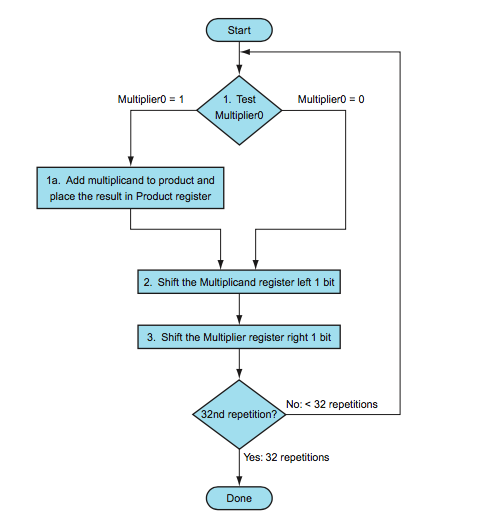
\includegraphics[scale = 0.75]{multalgorithm} $$ 

Booth's Algorithm \begin{itemize} 
\item For n bit signed point numbers 
\item n is the number of bits in the Multiplicand 
\item n is also the number of bits in the Multiplier
\item A is the left half of the Product Register 
\item Q is the right half of the Product Register 
\item Q$_0$ is the rightmost (least significant) bit of Q
\item Q$_{-1}$ is an extra bit to the right of Q
\item A and Q each have n bits 
\item Therefore the Product Register has 2n bits \end{itemize} 
$$ 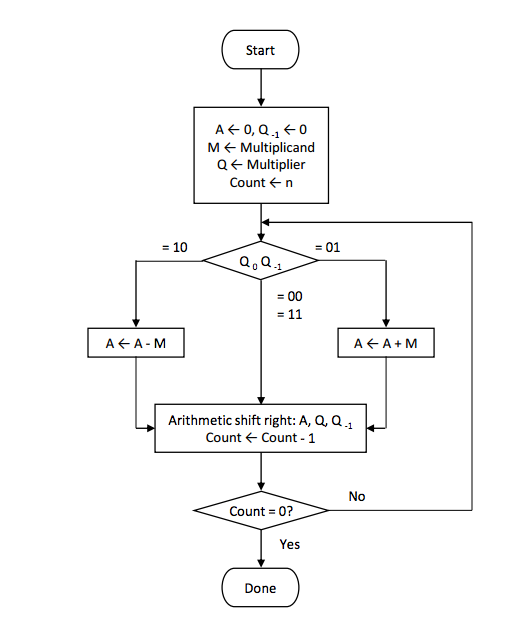
\includegraphics[scale = 0.5]{booth} $$ 

Division Algorithm \begin{itemize} 
\item For $n$-bit unsigned fixed point numbers 
\item The Remainder Register is $2n$ bits in length with the dividend placed in the right half and all zeros in the left half 
\item The Divisor Register is $2n$ bits in length with the divisor placed in the left half and all zeros in the right half 
\item The Quotient Register is $n$ bits in length initialized to all zeros \end{itemize}
$$ 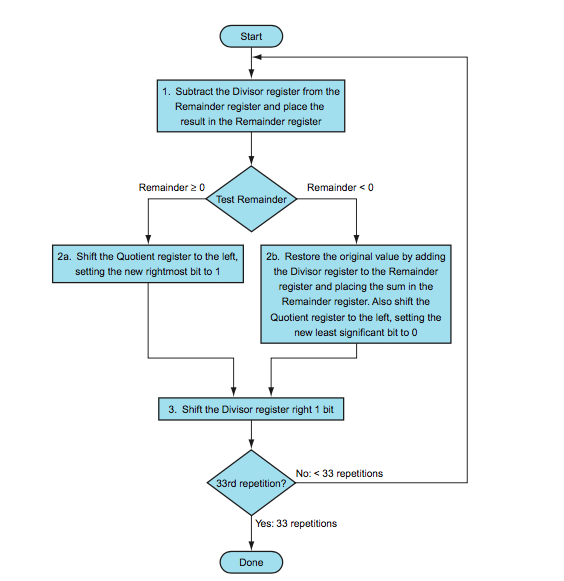
\includegraphics[scale = 0.75]{divisionalgorithm} $$ 
For Division of Signed Binary Integers 
\begin{itemize} 
\item If the signs of the operands (dividend and divisor) are different, the quotient is negative. 
\item If the signs of the operands are the same, the quotient is positive. \end{itemize} \newpage


\subsection{Floating Point Numbers (Fixed Point Numbers \\ with a Fractional Part)}
\begin{definition} Fixed $<w, b>$: defines the format of a fixed point number where $w$ is the total number of bits to represent the fixed point number and $b$ is the number of those $w$ bits which are to the right of the binary point. \end{definition} 
\begin{example} Binary fixed point numbers given with their format: \begin{itemize} 
\item 011.1, 011.0 and 100.1 have format fixed$<4,1>$ 
\item 11.00, 00.01 and 01.01 have format fixed$<4,2>$ 
\item 1100, 0001 and 0101 have format fixed$<4,0>$ 
\end{itemize} \end{example}
Two's complement implements signed fixed point numbers with a fractional part. \\~\\

Signed Binary Numbers in 4 Bits \\ $$\begin{tabular}{|c|c|c|c|c|c|c|c|c|} \hline 
Bit Combinations & 0000 & 0001 & 0010 & 0011 & 0100 & 0101 & 0110 & 0111 \\ \hline
Fixed$<4,1>$ & 0 & 0.5 & 1 & 1.5 & 2.0 & 2.5 & 3.0 & 3.5 \\ \hline
Fixed$<4,2>$ & 0 & 0.25 & 0.50 & 0.75 & 1.00 & 1.25 & 1.50 & 1.75 \\ \hline
Fixed$<4,0>$ & 0 & 1 & 2 & 3 & 4 & 5 & 6 & 7 \\ \hline  \end{tabular} $$ 

Signed Binary Numbers in 4 Bits \\ $$\begin{tabular}{|c|c|c|c|c|c|c|c|c|} \hline 
Bit Combinations & 1000 & 1001 & 1010 & 1011 & 1100 & 1101 & 1110 & 1111 \\ \hline
Fixed$<4,1>$ & -4 & -3.5 & -3 & -2.5 & -2 & -1.5 & -1 & -0.5 \\ \hline
Fixed$<4,2>$ & -2.00  & -1.75 & -1.50 & -1.25 & -1.00 & -0.75 & -0.50 & -0.25 \\ \hline
Fixed$<4,0>$ & -8 & -7 & -6 & -5 & -4 & -3 & -2 & -1 \\ \hline \end{tabular} $$ 
Conversion between the Integer Part Separately from the Fractional Part: \\~\\
Algorithm to convert a nonnegative integer fractional part from decimal to the binary, octal or hexadecimal number system: \begin{enumerate}
\item Initialize, num = ``fractional part''
\item Compute num = num $\cdot$ base 
\item Integer part of num is the next (binary, octal, hexadecimal) digit of the result 
\item Discard the integer part of num 
\item Repeat step 2 through 5 until num is zero \end{enumerate} 
Warning: num might not reach zero; in that case, repeat steps 2 through 5 until the result consists of a reasonable number of digits. \newpage
Algorithm to convert a nonnegative fractional part from binary, octal, or hexadecimal number system to decimal \begin{enumerate} 
\item Initialize, result = 0
\item For each digit from least to most significant, compute result = (result + digit) / base \end{enumerate} 

Algorithm to convert a nonnegative fractional part from binary, octal or hexadecimal number system to one of the other two number system \begin{enumerate}
\item Group fractional digits into groups of 2, 3 or 4 (binary, octal, hexadecimal respectively) and convert into integer values from left to right of the point
\item Convert the nonnegative integer fractional part attained into binary, octal or hexadecimal using algorithm previously written \end{enumerate} 
\begin{definition} Normalized Form: a number in scientific notation \end{definition}
\begin{definition} Denormalized: a floating number that has a 0 in the non-fractional part of the integer in scientific notation \end{definition}
Floating Point Binary Numbers (IEEE 754 standard) \begin{itemize} 
\item  Single Precision - 32 Bits - Bias value of 127 \begin{itemize} 
\item Signed  - 1 bit - 0 if positive, 1 if negative
\item Exponent - 8 bits - range: 126 to 127
\item Significand / Mantissa - 23 bits  \end{itemize} 
\item Double Precision - 64 Bits - Bias value of 1023 \begin{itemize}
\item Signed - 1 bit 
\item Exponent - 11 bits 
\item Significand / Mantissa - 52 bits \end{itemize} \end{itemize} 
\begin{example} Express 12.3125 in decimal into binary normalized. $$\begin{aligned} 
0.3125 \cdot 2 &= 0.625 \\
0.625 \cdot 2 &= 1.25 \\
0.25 \cdot 2 &= 0.5 \\
0.5 \cdot 2 &= 1.0 \end{aligned} $$ 
12.3125 in binary is (1100.0101). 
$$ 1100.0101 \cdot 2^0 = 1.1000101 \cdot 2^3 $$  
In single precision, the significand is 10010100.. The exponent bit is 127 + 3 = 130 or 10000010. The sign bit is 0. 
Thus 12.3125 is 01000001010010100 in binary form. \end{example} 
Note: To move the point to the right, decrease the exponent; to move the point to the left, increase the exponent. \\~\\
IEEE 754 encoding of floating point numbers (a separate sign bit determines the sign.) 
$$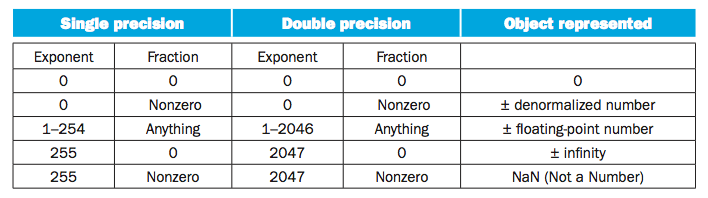
\includegraphics[width = \textwidth]{precisions}$$ 
Floating Point Arithmetic Operations \begin{itemize} 
\item Addition or Subtraction \begin{enumerate} 
\item In order to add the two numbers, the exponents of the two numbers need to be the same. Convert the number with the smaller exponent to the equivalent number whose exponent is the same as the other number. 
\item Add or subtract the mantissa of the two numbers 
\item Normalize the result 
$$ 1.110 \cdot 2^2 + 1.000 \cdot 2^0 = 1.110 \cdot 2^2 + 0.01 \cdot 2^2 = 10.000 \cdot 2^2 = 1.0000 \cdot 2^3 $$
\end{enumerate} 
\item Overflow and Underflow \begin{itemize} 
\item Overflow occurs when the result of a floating point operation is larger than the largest positive value or smaller than the smallest negative value; in other words, the magnitude (exponent) is too large to represent 
\item Underflow occurs when the result of a floating point operation is smaller than the smallest positive value or larger than the largest negative value; in other words, the magnitude (exponent) is too small to represent \end{itemize} 
\item Multiplication \begin{enumerate}
\item Add the exponents; if the exponents are in biased form, then subtract the bias from the sum 
\item If exponent overflow or underflow, then report and stop 
\item Multiply the significands considering their signs 
\item Normalize the result 
\item Round the result \end{enumerate}
\item Division \begin{enumerate} 
\item Subtract the exponents; if the exponent is in biased form, then add the bias to the difference 
\item If exponent overflow or underflow, then report and stop 
\item Divide the significands 
\item Normalize the result 
\item Round the result \end{enumerate} 
\end{itemize} 



\section{MIPS Assembly Language Programming}
\subsection{MIPS Assembly Language Programming}

MIPS Subroutines: subprograms (procedure, function, method) 
\begin{definition} Subroutines: a tool programmers use to structure programs to both to make them easier to understand and to allow code to be reused \end{definition}

Each subroutine is placed after the main section of the program, one after another. Each starts with a label and ends with a jr \$ra. 


The Steps Needed for the Execution of a Subroutine: \begin{enumerate} 
\item Put parameters in a place where the subroutine can access them. 
\item Transfer control to the subroutine. 
\item Acquire the storage resources needed for the subroutine. 
\item Perform the desired task. 
\item Put the result value in a place where the calling (sub)program can access it. 
\item Return control to the point of origin, since a subroutine can be called from several points in a program. \end{enumerate} 

Subroutine Resources \begin{itemize} 
\item Registers used for calling subroutines \begin{itemize} 
\item \$a0 - \$a3: Four argument registers in which to pass parameters 
\item \$v0 - \$v1: Two value registers in which to return values 
\item \$ra: One return register to return to the point of origin  \end{itemize} 

\item The jump-and-link instruction (jal) jumps to an address and simultaneously saves the address of the following instruction in register \$ra
\item At the end of a subroutine, the jump register jr is used at the end of a subroutine to return to the calling (sub)program, jr \$ra 
\end{itemize} 

Program in C++: \\ int leafExample(int g, int h, int k, int j)\{
\indent int f; \\
\indent if (i == j) f = g + h \\
\indent else f = g - h \\
\indent return f;  \\
\} \\~\\
Program in MIPS:

\$a0 $\to$ g \\ \$a1 $\to$ h, \$a2 $\to$ i, \$a3 $\to$ j, \$s0 $\to$ f \\ 
b \$a2, \$a3, else \\
bne \$a2, \$a3 \\ add \$s0, \$a0, \$a1 \\
j endif \#only needed if there's an else statement \\
else sub \$s0, \$a0, \$a1 \\ 
endif: \\ 

 \noindent leafExample: \\
\indent bne \#a2, \#a3, else \\
 \indent add \$s0, \$a0, \$a1 \\
 \indent j endif \\
 else sub \$s0, \$a0, a1 \\ 
 endif move \$v0, \$s0 \\ 
 \indent jr \$ra \\~\\

MIPS Runtime Stack \begin{itemize} 
\item Often, a subroutine does call either subroutine or even itself. 
\item Therefore, to ensure the program and all called subroutines work properly, registers used by the current called subroutine need to be saved before the current called subroutine can begin executing its own code. 
\item The runtime stack and the Stack Pointer register \$sp are the tools for saving register contents 
\item Stack is implemented LIFO  

\end{itemize} 











Program in C++: \\ int leafExample(int g, int h, int k, int j)\{
\indent int f; \\
\indent f = (g + h) - (i + j); \\
\indent return f;  \\
\} \\~\\


Program in MIPS
 \noindent leafExample: \\
 \indent pushes \\
 \indent add \$s0, \$a0, \$a1 \\
 \indent add \$t0, \$a2, \$a3 \\ 
 \indent  sub \$s0, \$t0, t1 \\ 
 \indent move \$v0, \$s0 \\ 
 \indent pop \\
 \indent jr \$ra \\~\\
 
  
 
 int leafExample(int g, int h, int i, int j) {
 int f; 
 f = (g + h) - (i + j); 
 return f; 
 }
 
 \$a0 - g. \$a1 - h, \$a2 - i, \$a3 - j \\
 
In MIPS with Stack: \\ 
leafExample \\
addi \$sp, \$sp, 0 \\
sw \$t1, 8(\$sp) \\ 
sw \#t0, 4(\$sp) \\ 
sw \$ \\~|\

At the Beginning of a Subroutine: \begin{itemize} 
\item the \$sp register starts at a high address and moves towards lower addresses 
\item To push registers onto the stack, subtract (the number of registers times 4) from \$sp 
\item 
\item Remove each register from the stack 
\item Add (the number of registers times 4) to \$sp 
\end{itemize} 

Register Saving Conventions for MIPs Programmers \begin{itemize} 
\item Caller (sub)program - the main part of the program or subroutine calling another subroutine 
\item Callee subroutine - the subroutine called 
\item If the callee uses temporary registers (\$t0 - \$t9), it is the caller (sub)program which should save them on this stack 
\item If the callee uses saved registers (\$s0, \$s7), it is the callee subroutine which should save them on the stack 

\end{itemize} 

Recursion 
\begin{itemize} 
\item Often, a subroutine does call other subroutine and even itself 
\item Therefore, the callee subroutine needs to store the argument registers it uses as well as the return address in \$ra onto the stack 

\end{itemize}

\subsection{MIPS Architecture}

\subsection{MIPS ALU Design}

MIPS Datapath Diagram
$$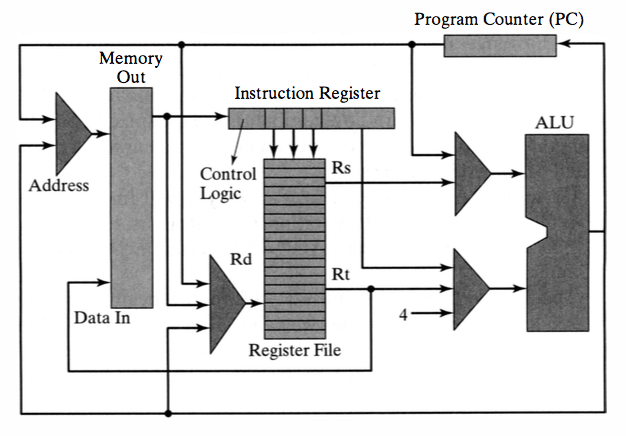
\includegraphics[scale = 0.5]{mipsdatapath}$$ 
Register File 
$$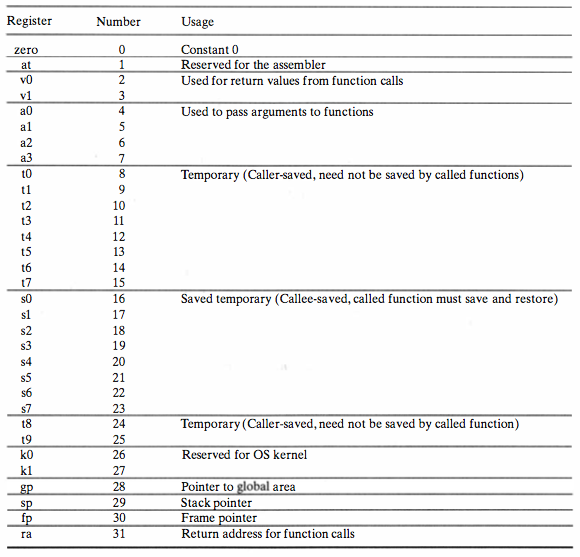
\includegraphics[scale = 0.75]{registerfile}$$ 
Note: All registers have a \$ in front of it. 
\begin{definition}.data represents the memory area of the program \end{definition} 
\begin{definition}.text: code area of the program \end{definition}
Assembler Directives: \\ 
Macros: \\ 
Syntax for MIPS Assembly Language Instructions: 
\begin{center} [label:] Op-code [operand,] [operand,] [Operand] [\#command]  \end{center}
The first operand is usually the destination and the others are sources. \newpage
Types of R format: Op-code \$rd, \$r \begin{itemize}
\item add \$rd, \$rs, \$rt 
\item addu (unsigned) \$rd, \$rs, \$rt
\item addi (immediate, numerical literal): \$rd, \$rs, Imm
\item addiu (immediate unsigned): \$rd, \$rs, Imm 
\item sub \$rd, \$rs, \$rt 
\item subu (unsigned) \$rd, \$rs, \$rt
\item and: \$rd, \$rs, \$rt 
\item or: \$rd, \$rs, \$rt
\item XOR (exclusive or): \$rd, \$rs, \$rt
\item NOR:  \$rd, \$rs, \$rt
\item mult: \$rd, \$rs, \$rt (64 bits)
\item mfhi: \$rd - get upper half of product
\item mfo: \$rd - get lower half of product
\item div: \$rs, \$rt
\item divu (unsigned): \$rs, \$rt
\item mfhi: \$rd - get remainder
\item mflo \$rd - get quotient 
\end{itemize}

Types of I Format - Data Transfer \begin{itemize} 
\item lw (load word): \$rt, offset(\$rs)
\item sw (store word): \$rt, offset(\$rt)
\end{itemize} 

A word is a certain number of bits. A byte is composed of 8 bits. 
In MIPS, a word is 32 bites, or 4 bytes. 
Variables are represented as .word, each 4 bytes. 
The first variable's address is 0; the next one's address is 4, the next one's address is 8, etc. 
The memory address is found by adding \$rs and offset. 
Main is represented as .text \\~\\
Macro Instructions \begin{itemize} 
\item Load Address la: \$rs, Label
\item Load Immediate li: \$rs, Imm
\end{itemize}

Conditional Branches in I Format \begin{itemize} 
\item Branch If Equal beq: \$rs, \$rs, Label
\item Branch if Not Equal bne: \$rs, Label

\end{itemize} 

J Format \begin{itemize} 
\item Jump j: Label
\item Jump and Link jal: Label
\item Jump and Link Register jalr: \$rd, \$rs
\item Jump Register jr: \$rs 
\end{itemize} 

Input and Output \begin{itemize} 
\item Read an integer: \\ li \$v0, 5 \\ syscall \\ \#The integer read in is placed in register \$v0
\item Print an integer: \\ \$v0, a0 \\ li \$v0, 1 \\ syscall \\ \# Place the integer to print in register \$a0
\item Read a String: \\ \# Place the address of the string's storage into register \$a0. Place the maximum number of chars to read in into register \$a1 \\ la \$a0, myString \\ li, \$a1, 100 \\ li, \$10, 8 \\ syscall
\item Print a String: \\ la \$a0, inputPrompt \\ li, \$v0, 4 \\ syscall \\ \# Place the address of the string's storage into register 
\end{itemize}

String Literal \begin{itemize} 
\item .ASCII 
\item .ASCIIz - null terminated - add a 0 after the least character in a string 
\item new line \textbackslash n  
\end{itemize}

String Variables \begin{itemize} 
\item .space n - allocates $n$ number of bytes for storage (use one additional byte for null) \\ myString .space 101 
\end{itemize}  

\noindent Vector - Arrays \\ \# an array of Integers \\ C: .space n \\ 
\# n must be a multiple of 4 \\
Note: The memory address is \$rs + offset. Therefore \\
lw \$rt, offset(\$rs) will load a value into the array. \\
sw \$sw, \$rt, offset(\$rt) will save a value into the array \\~\\
Branch of Equal: beq \$rs, \$rd, Label \\ 
Branch of not Equal: bne \$rs, \$rd, Label \\ 
Set if Less than: slt, \$rd, \$rs, \$rt \\
if rs $>$ rt, then the first operand gets a value of 1, else 0 \\
Branch if less than: ble, \$rd, \$rs, \$rt  \\ 

\subsection{Algorithm Development in Pseudocode}

\section{Combinational Logic} 
Logic Design \\
Boolean Values: 0, 1 - boolean literals \\~\\

Binary Values \begin{itemize} 
\item High voltage - true, 1, or asserted 
\item Low voltage - false, 0, or deasserted \end{itemize} 

Logic Blocks \begin{itemize} 
\item Logic Blocks are categorized as one of two types based on whether or not the block contains memory 
\item Combinational Logic Blocks: logic blocks without memory using the processes of combinational logic; the output of a combinational logic block depends only on it current inputs 
\item Sequential Logic Blocks: logic blocks with memory using the processes of sequential logic; the output of a sequential logic block can depend on both the inputs and the value stored in memory, which is called the state of the logic block 
\end{itemize} 

Truth Tables \begin{itemize} 
\item A table to define the output value for each combination of the inputs 
\item For a logic block of $n$ inputs, there are $2^n$ entries in the truth table 
\item Defines any combinational logic block but grows in size quickly 
\item A shorthand lists only the input combinations which have an output value of 1 

\end{itemize}

Boolean Logic \begin{itemize} 
\item Developed by George Boole, a nineteenth century English Mathematician 
\item Defines a combinational logic block using logic equations and Boolean algebra 
\item All inputs and outputs (Boolean variables) have a value of 0 or 1 
\item Three Boolean Opeartors \begin{enumerate} 
\item OR: written as +; the result of OR is 1 if either input is 1; it is also called logical sum 
\item AND: written as $\cdot$: the result of AND is 1 only if both values are 1; it is also called logical product
\item NOT: written as $\bar{A}$: the result of NOT is 1 if the input value is 0 and is 0 if the input value is 1; the NOT operator produces the negation or inversion of the input value 
\end{enumerate} 
\end{itemize}

$$ \begin{tabular}{|c|c|c|c|c|c|} \hline
$A$ & $B$ & $A + B$ &  $A \cdot B$ & $\overline{A}$ & $\overline{B}$ \\ \hline
0 & 0 & 0 & 0 & 1 & 1 \\ \hline
0 & 1 & 1 & 0 & 1 & 0 \\ \hline
1 & 0 & 1 & 0 & 0 & 1 \\ \hline
1 & 1 & 1 & 1 & 0 & 0 \\ \hline
\end{tabular} $$ 

Boolean Algebra Laws \begin{itemize} 
\item Identify Law: $A + 0 = A$ and $A \cdot 1 = A$ 
\item Zero and One Law: $A \cdot 0 = 0$ and $A + 1 = 1$
\item Inverse Law: $A  + \bar{A} = 1$ and $A \cdot \bar{A} = 0$ 
\item Commutative Laws: $A + B = B + A$ and $A \cdot B = B \cdot A$ 
\item Associative Laws: $A + (B + C) = (A + B) + C$ and $A \cdot (B \cdot C) = (A \cdot B) \cdot C$ 
\item Distributive Laws: $A \cdot (B + C) = (A \cdot B) + (A \cdot C)$ and $A + (B \cdot C) = (A + B) \cdot (A + C)$ 
\item DeMorgan's Law: $\overline{A + B} = \bar{A} \cdot \bar{B}$ and $\overline{A \cdot B} = \bar{A} + \bar{B}$ 
\end{itemize} 

\begin{example} 
$$\begin{aligned} (\bar{x} \cdot \bar{y} \cdot z) + (\bar{x} \cdot y \cdot z) + (x \cdot \bar{y}) &= (\bar{x} \cdot z \cdot  \bar{y}) + (\bar{x} \cdot z \cdot y) + (x \cdot \bar{y}) \\ &= ((\bar{x} \cdot z) \cdot \bar{y}) + ((\bar{x} \cdot z) \cdot y) + (x \cdot \bar{y}) \\ &= (\bar{x} \cdot \bar{z}) \cdot (\bar{y} + y) + (x \cdot \bar{y}) \\ &= (\bar{x} \cdot z) \cdot (1) + (x \cdot \bar{y}) \\ &= (\bar{x} \cdot z) + (x + \bar{y}) \\ (\bar{x} \cdot \bar{y} \cdot \bar{z}) + (\bar{x} \cdot y \cdot \bar{z}) + (x \cdot \bar{y} \cdot \bar{z}) + (x \cdot y \cdot \bar{z}) &= \Big((\bar{x} \cdot \bar{y}) + (\bar{x} + y) + (x + \bar{y}) + (x + y)\Big) \cdot \bar{z} \\ &= \Bigg(\Big(\bar{x} \cdot (\bar{y} + y)\Big) + \Big(x \cdot (\bar{y} + y)\Big)\Bigg) \cdot \bar{z} \\ &= \Big( (\bar{x} \cdot 1) + (x \cdot 1)\Big) \cdot \bar{z} \\ &= (\bar{x} + x) \cdot \bar{z} \\ &= 1 \cdot \bar{z} \\ &= \bar{z}  \end{aligned} $$ \end{example} 

\begin{example} 
$$ A + (A \cdot B) = (A \cdot 1) + (A \cdot B) = A \cdot (1 + B) = A \cdot 1 = A $$ 
$$A \cdot (A + B) = (A + 0) \cdot (A + B) = A + (0 \cdot B) = A + 0 = A $$ 
\end{example} 

Operator Precedence: NOT, AND, OR \\~\\ 

Logic Gates \begin{itemize} 
\item And Gate (capital D with 2 inputs and 1 output): implements the And logical operator 
\item Or Gate (curved capital D with 2 inputs and 1 output): implements the Or logical operator 
\item Not Gate (triangle followed by small circle with 1 input and 1 output): implements the Not logical operator, also called inverter 


 \end{itemize} 

Functional Completeness: \begin{itemize} 
\item The original set of Boolean operations is (And, Or, Not) 
\item A set of Boolean operators is functionally complete if all other Boolean operators can be constructed from this set 
 \item The set of Boolean operators (And, Not) is functionally complete
 \item Because, the OR operator can be defined in terms of And and Not
 \item How? Using two Boolean properties \begin{itemize} 
  \item Double negation \item DeMorgan's Law 
  \item $\overline{A \cdot B} = \bar{A} + \bar{B} $ \end{itemize}
  \item $\overline{\bar{A} \cdot \bar{B}} = \bar{\bar{A}} + \bar{\bar{B}} = A + B $ 
  \item This set of Bollean operation (Or, Not) is functionally complete 
  \item Because, the And operator can be defined in terms of Or and Not 
  \item How? Using 2 Boolean operations \begin{itemize} 
  \item Double Negation $\bar{\bar{A}} = A $ 
  \item DeMorgan's Law $\overline{A + B} = \bar{A} \cdot \bar{B} $ \end{itemize} 
  \item $ \overline{\bar{A} + \bar{B}} = \bar{\bar{A}} \cdot \bar{\bar{B}} = A \cdot B $ \end{itemize}

Exclusive OR ($\oplus$, double curved capital D): returns a 1 if both values are different or a 0 if both values are the same 
$$ A \oplus B = (\bar{A} \cdot B) + (A \cdot \bar{B}) $$ 
$$\begin{tabular}{|c|c|c|c|} \hline
$A$ & $B$ & $A + B$ & $A \oplus B$ \\ \hline 
0 & 0 & 0 & 0 \\ \hline
0 & 1 & 1 & 1 \\ \hline
1 & 0 & 1 & 1 \\ \hline 
1 & 1 & 1 & 0 \\ \hline \end{tabular} $$ 

Logic Gates: \begin{itemize} 

\item Nand Gate (capital D followed by a small circle, has 2 input an 1 output): $\overline{A \cdot B}$; is a functionally complete set
\item Not Gate: implemented using a Nand gate (square, capital D, small circle; has 1 input and 1 output) 

$$ \begin{tabular}{|c|c|c|cl} \hline 
$A$ & $A$ & $A \cdot A$ & $\overline{A \cdot A}$ \\ \hline 
0 & 0 & 0 & 1 \\ \hline 
1 & 1 & 1 & 0 \\ \hline
\end{tabular} $$ 

\item And gate implemented using Nand gates (capital D, small circle followed by a square, capital D and small circle; 2 input and 1 output) $A$ NAND $B$ = $ \overline{A \cdot B} $ 

\item Or gate implemented using Nand gates (for each input, 1 square, capital d, small circle to a capital D followed by a small circle, 1 output) $\bar{A}$ NAND $\bar{B} = \overline{\bar{A} \cdot \bar{B}} = \bar{\bar{A}} + \bar{\bar{B}} = A + B $ 

\item Nor Gate: $\overline{A  + B}$, functionally complete set (2 inputs into a curved D followed by a small circle) 

\item Not Gate implemented using a Nor gate (square, curved D, small circle) 

\item Or Gate implemented using Nor gates (2 inputs into a curved D, small circle giving 1 output which goes into a square, curved D and a small circle)

\item And Gate implemented using Nor Gates (2 of square, curved d, small circles into a curved D and small circle, 1 output)

\end{itemize} $$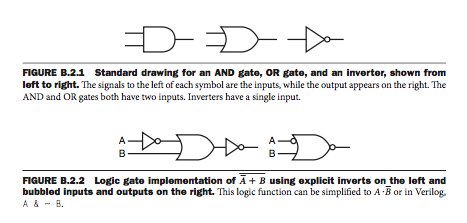
\includegraphics[width = \textwidth]{gates}$$ 

Decoder \begin{itemize} 
\item Decoder: a combinational logic circuit that converts a binary integer value to an associated pattern of output bits 
\item For the decoders discussed in this class, only output bit is asserted for each binary integer input value 
\item With $n$ inputs, the decoder has $2^n$ outputs 
\item They are used in a wide variety of applications, including data demultiplexing, seven segment displays and memory address decoding 
\item A 3 to 8 decoder has 3 inputs and up to 8 outputs $$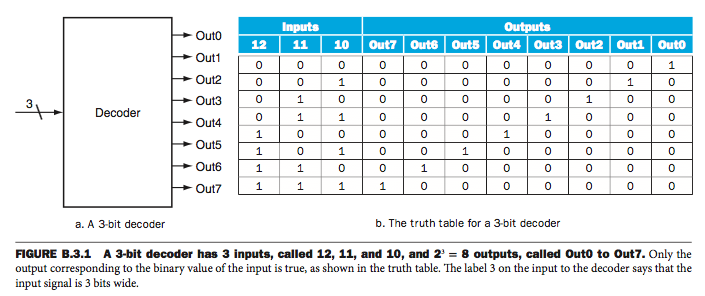
\includegraphics[width = \textwidth]{3bitdecoder}$$  \end{itemize}

Simple Encoder \begin{itemize} 
\item A simple encoder circuit is a one-hot to binary converter. That is, if there are $2^n$ input lines, and at most only one of these will ever be asserted, the binary code of this `hot' line is produced on the $n$-bit output lines 
\item Works the opposite of a decoder
\item 8 to 3 Encoder - works the opposite as where the 8 outputs on the right are inputs and the 3 inputs on the left are outputs
\end{itemize} 

Multiplexer \begin{itemize} 
\item Called a selector because its output is one of the inputs selected by a control, selector bit(s); only has one output
\item 2 to 1 Multiplexer  $$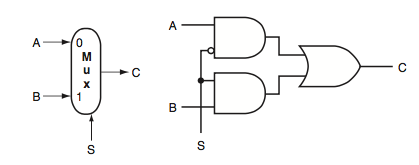
\includegraphics[width = \textwidth]{multiplexer} $$ 
\end{itemize} 

$N$-Bit Multiplexer \begin{itemize} 
\item An $n$-input multiplexer needs $\lceil \log_2 n \rceil$ selector (control) bits 
\item The multiplexer consists of \begin{itemize} 
\item A decoder with $n$ outputs signals, each matched to a unique multiplexer input
\item An array of $n$ AND gates, each combining one of the multiplexers inputs with an output signal from the decoder 
\item A single large OR gate which combines the outputs of the AND gates 
\end{itemize} 
\item The multiplexer inputs are numbered from 0 to $n - 1$ 
\item The selector bits represents a binary number 
\item Each selector bit binary combination selects the multiplexer input corresponding to the binary number represented by that selector bit binary combination 
\item The currently selected multiplexer input connects to the multiplexer output 
\item If the selector bits changes, then the multiplexer input connected to the multiplexer output changes 
\end{itemize} 
4 to 1 Multiplexer
$$\begin{tabular}{|c|c|c|c|c|} \hline 
& Inputs & & Outputs \\ \hline
A & B & C & D & E \\ \hline
0&0&0&0&0 \\ \hline 
0&0&0&1&0 \\ \hline 
0&0&1&0&1 \\ \hline 
0&0&1&1&1 \\ \hline 
0&1&0&0&1 \\ \hline 
0&1&0&1&0 \\ \hline 
0&1&1&0&0 \\ \hline 
0&1&1&1&1 \\ \hline 
1&0&0&0&0 \\ \hline 
1&0&0&1&1 \\ \hline 
1&0&1&0&1 \\ \hline 
1&0&1&1&1 \\ \hline 
1&1&0&0&0 \\ \hline 
1&1&0&1&0 \\ \hline 
1&1&1&0&1 \\ \hline 
1&1&1&1&0 \\ \hline \end{tabular} $$ 


Karnaugh Maps (K-Maps) \begin{itemize} 
\item Used to generate a simplified version of the sum of products expressions of a logic function 
\item Kmap for 3 inputs 
$$\begin{tabular}{|c|c|c|c|} \hline \\ 
& Inputs & & Output \\ \hline 
A & B & C & D \\ \hline 
0&0&0&0 \\ \hline 
0&0&1&0 \\ \hline 
0&1&0&1 \\ \hline 
0&1&1&1 \\ \hline 
1&0&0&1 \\ \hline 
1&0&1&0 \\ \hline 
1&1&0&1 \\ \hline 
1&1&1&1 \\ \hline \end{tabular} $$ 
\item Kmap for 4 inputs 
$$\begin{tabular}{|c|c|c|c|c|} \hline 
& Inputs & & & Outputs \\ \hline
A & B & C & D & E \\ \hline
0&0&0&0&0 \\ \hline 
0&0&0&1&0 \\ \hline 
0&0&1&0&0 \\ \hline 
0&0&1&1&0 \\ \hline 
0&1&0&0&0 \\ \hline 
0&1&0&1&0 \\ \hline 
0&1&1&0&1 \\ \hline 
0&1&1&1&0 \\ \hline 
1&0&0&0&1 \\ \hline 
1&0&0&1&1 \\ \hline 
1&0&1&0&1 \\ \hline 
1&0&1&1&1 \\ \hline 
1&1&0&0&1 \\ \hline 
1&1&0&1&1 \\ \hline 
1&1&1&0&1 \\ \hline 
1&1&1&1&1 \\ \hline \end{tabular} $$  \end{itemize} 

In K-maps, the size of rectangles of 1s must be powers of 2 (1, 2, 4, 8, etc) that don't have to be right next to each other but can overlap. Bigger size is better. Using less inputs is also better. Each rectangle gets a term and whichever input has all 1s goes in the equation. \\ Simplified form of Sum of Products for $E$: 
$$E = ( A \cdot C ) + ( A \cdot \bar{B} ) + ( B \cdot C \cdot \bar{D} ) $$ 


Two Level Logic \begin{itemize} 
\item Any logic function can be written as a logic equation in its canonical form where each input variable can be written as itself ad its complement ($A, \bar{A}$) and there are only two levels of operators, one being AND and the other being OR 
\item This form is a two-level representation and there are two versions: \begin{itemize} 
\item Sum of Products: a logical sum (OR) of products, product terms 
\item Product of Sums: a logical product (AND) of sums, sum terms 
\end{itemize} \end{itemize} 

Logic Function $$\begin{tabular}{|c|c|c|c|c|c|} \hline 
& Inputs & & & Outputs & \\ \hline 
A & B & C & D & E & F \\ \hline 
0&0&0&0&0&0 \\ \hline 
0&0&1&1&0&0 \\ \hline
0&1&0&1&0&0 \\ \hline 
0&1&1&1&1&0 \\ \hline 
1&0&0&1&0&0 \\ \hline 
1&0&1&1&1&0 \\ \hline 
1&1&0&1&1&0 \\ \hline 
1&1&1&1&0&1 \\ \hline \end{tabular} $$ 
$D$ is true if at least 1 input is true; E is true if exactly 2 inputs are true; F is true only if all 3 inputs are true. \\~\\
$$ \begin{aligned} D &= (\bar{A} \cdot \bar{B} \cdot C) + (\bar{A} \cdot B \cdot \bar{C}) + (\bar{A} \cdot B \cdot C) + (A \cdot \bar{B} \cdot \bar{C}) + (A \cdot \bar{B} \cdot C) + (A \cdot B \cdot \bar{C}) + (A \cdot B \cdot C) \\ &= 001 ~~010 ~~011 ~~100 ~~101 ~~110 ~~111 \\ &= (A + B + C) \\ &= 000 \\ E &= (A + B + C) \cdot (A + B + \bar{C}) \cdot (A + \bar{B} + C) \cdot (\bar{A} + B + C) \cdot (\bar{A} + \bar{B} + \bar{C}) \\ &= 000 ~~001 ~~010 ~~100 ~~111 \\ &= (\bar{A} \cdot B \cdot C) + (A \cdot \bar{B} \cdot C) + (A \cdot B \cdot \bar{C}) \\ &= 011 ~~101 ~~110 \\ F &= (A \cdot B \cdot C) \end{aligned} $$ 

Sum of Products \begin{itemize} 
\item Construct the sum of products logic equation from the logic function's truth table 
\item Each truth table entry whose output value is 1 is a product term in the sum of products equation 
\item A product term is also called a minterm 
\item A product term is the logic product of all the input variables where the input variable is itself ($A$) if its value in the truth table is 1 or the complement of itself ($\bar{A}$) if its value in the truth table is 0 
\item The logic function's sum of products equation is also called the logical sum of minterms 
\end{itemize} 

Product of Sums \begin{itemize} 
\item Construct the product of sums logic equation from the logic functions's truth table 
\item Each truth table entry whose output value is 0 is a sum term in the product of sums equation 
\item A sum term is also called a maxterm 
\item A sum term is the logic sum of all the input variables where the input variable is itself ($A$) if its value in the truth table entry is 0 or the complement of itself ($\bar{A}$) if its value n the truth table entry is 1 
\item The logic function's product of sums equation is also called the logical product of its maxterms 
\end{itemize} 


%An Example Logic Function Truth Table (insert from picture) $$\begin{tabular}{|c|c|c|c|c|c|} \hline 
%Input & & & Output & &  \\ \hline 
%A & B & C & D & E & F \\ \hline
%0&0&0&0&0&0 \\ \hline
%0&0&1&1&0&0 \\ \hline
%0&1&0&1&0&0 \\ \hline
%0&1&1&1&1&0 \\ \hline
%1&0&0&1&0&0 \\ \hline
%1&0&1&1&1&0 \\ \hline
%1&1&0&1&1&0 \\ \hline
%1&1&1&1&0&1 \\ \hline \end{tabular} $$ 

%Insert DEF from picture.

Sum of Products: 
$$ G = (\bar{A} \cdot B \cdot \bar{C}) + (A \cdot \bar{B} \cdot \bar{C}) + (A \cdot B \cdot \bar{C}) $$
$$ G = 010 100 110$$
If this was product of sums, invert the 0s and 1s and puts the 1s in those rows. 
$$ H = (\bar{A} + B + \bar{C}) \cdot (A + \bar{B} + \bar{C}) \cdot (A + B + \bar{C}) $$ 
$$ H = 101 011 001 $$ 

$$ \begin{tabular}{|c|c|c|c|cl} \hline 
A&B&C&G& H \\ \hline  
0&0&0&0&0 \\ \hline 
0&0&1&0&1 \\ \hline
0&1&0&1&0 \\ \hline
0&1&1&0&1 \\ \hline 
1&0&0&1&0 \\ \hline
1&0&1&0&1 \\ \hline
1&1&0&1&0 \\ \hline
1&1&1&0&0 \\ \hline \end{tabular} $$ 


 PLA Integrated Circuit \begin{itemize} 
 \item Programmable Logic Array (PLA): a common structured logic implementation of the sum of products representation of a logic function 
 \item A PLA has a et of inputs and the corresponding inputs complements (implemented with a set of inverters) and two stages of logic 
 \item The first stage is an array of AND gates that form the set of product terms (minterms) 
 \item The second stage is an array of OR gates, each of which forms a logical sum of any number of the product terms 
 $$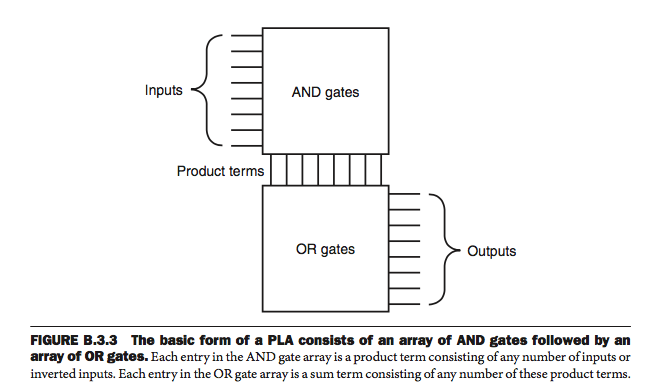
\includegraphics[width = \textwidth]{plabasic}$$ 
 
 \end{itemize} 
PLA Logic Circuit Representation Figure 
$$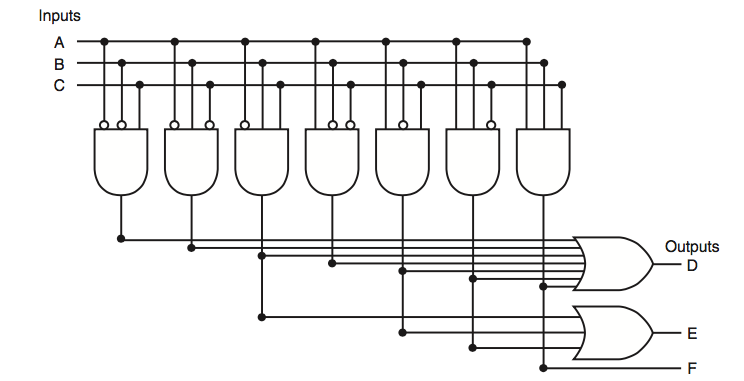
\includegraphics[width = \textwidth]{pla}$$ 

Alternative Diagram: vertical line represents minterm
$$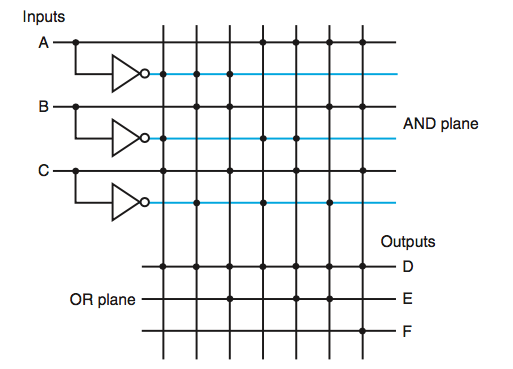
\includegraphics[scale = 0.5]{altpla}$$ 

Read-Only Memory (ROM): \begin{itemize} 
\item $m$ inputs, $2^m$ outputs 
\item The $m$ inputs are treated as the address to a entry 
\end{itemize} 

Half Adder Truth Table $$\begin{tabular}{|c|c|c|c|} \hline 
Input & & Output & \\ \hline 
A & B & $C_{out}$ & S \\ \hline 
0&0&0&0 \\ \hline 
0&1&0&1 \\ \hline 
1&0&0&1 \\ \hline 
1&1&1&0 \\ \hline
\end{tabular} $$ 

Half Adder Equations: $$ \begin{aligned} 
C_{out} &= A \cdot B \\ S &= \bar{A} \cdot B + A \cdot \bar{B} \\ &= A \oplus B
\end{aligned} $$  

Half Adder Circuit $$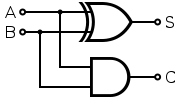
\includegraphics[width = \textwidth]{halfadder} $$

Full Adder Truth Table $$ \begin{tabular}{|c|c|c|c|c|} \hline 
& Input & & Output & \\ \hline 
A& B& $C_{in}$ & $C_{out}$ &S \\ \hline 
0&0&0&0&0 \\ \hline
0&0&1&0&1 \\ \hline
0&1&0&0&1 \\ \hline
0&1&1&1&0 \\ \hline
1&0&0&0&1 \\ \hline
1&0&1&1&0 \\ \hline
1&1&0&1&0 \\ \hline
1&1&1&1&1 \\ \hline \end{tabular} $$ 
$$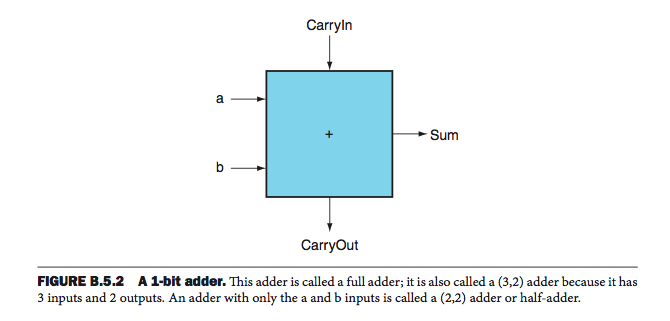
\includegraphics[width = \textwidth]{1bitadder}$$ 
$$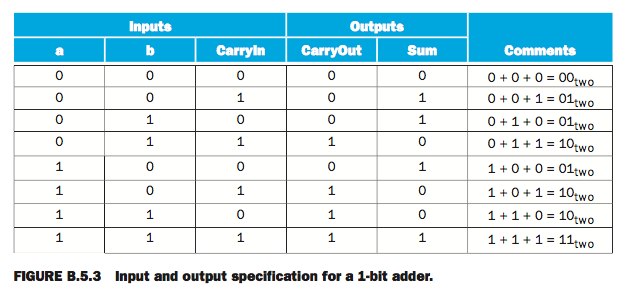
\includegraphics[width = \textwidth]{1bitaddertable}$$ 
$$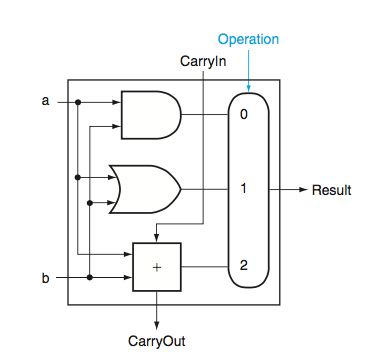
\includegraphics[width = \textwidth]{1bitALU3operations}$$ 
$$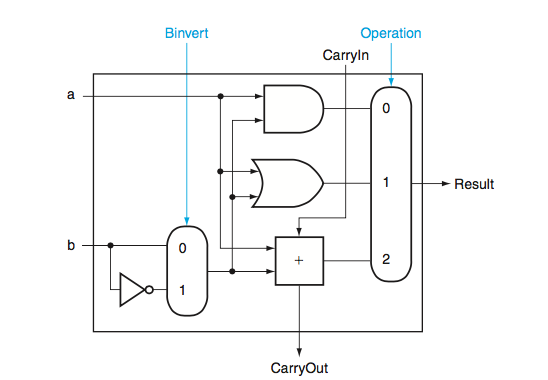
\includegraphics[width = \textwidth]{1bitALU4operations}$$ 




Full Adder Equations $$\begin{aligned} 
S &= (\overline{C_{in}} \cdot \bar{A} \cdot B) + (\overline{C_{in}} \cdot A \cdot \bar{B}) + (C_{in} \cdot \bar{A} \cdot \bar{B}) + (C_{in} \cdot A \cdot B) \\ &= \overline{C_{in}} \cdot ((\bar{A} \cdot B) + (A \cdot \bar{B})) + C_{in} \cdot ((\bar{A} \cdot \bar{B}) + (A \cdot B)) \\ &= \overline{C_{in}} \cdot (A \oplus B) + C_{in} \cdot (\overline{A \oplus B}) \\
C_{out} &= (\overline{C_{in}} \cdot A \cdot B) + (C_{in} \cdot \bar{A} \cdot B) + (C_{in} \cdot A \cdot \bar{B}) + (C_{in} \cdot A \cdot B) \\ &= (\overline{C_{in}} \cdot A \cdot B) + (C_{in} \cdot A \cdot B) + (C_{in} \cdot \bar{A} \cdot B) + (C_{in} \cdot A \cdot \bar{B}) \\ &= (\overline{C_{in}} + C_{in}) \cdot (A \cdot B) + C_{in} \cdot ((\bar{A} \cdot B) + (A \cdot \bar{B})) \\ &= 1 \cdot (A \cdot B) + C_{in} \cdot (A \oplus B) \\ &= (A \cdot B) + C_{in} \cdot (A \oplus B) \\ &= (A \cdot B) + C_{in} \cdot (A + B) \end{aligned} $$  


Full Adder Circuit \begin{itemize} 
\item Full Adder Block Box: 2 inputs and carry in into a box while carry out and sum leaves; adds 2 1 bit numbers 
\item Ripple Carry Adder: multiple full adder block boxes put together so that multiple numbers can be added together \end{itemize} 
 
 Propagation Delay \begin{itemize} 
 \item Propagation decay, or gate decay: The length of time which starts when the input to a logic gate becomes stable and valid to change, to the time that the output of that logic gate is stable and valid to change 
\item Measured as length of time or number of gates 
\item In a ripple carry adder circuit, sdd up propagation delay gates for each output in the direction it is traveling in 
\end{itemize} 


Carry Propagation \begin{itemize} 
\item $C_{out} = (A \cdot B) + C_{in} \cdot (A + B) $
\item $G = A \cdot B$ is called the carry generate term 
\item If $A$ and $B$ are 1 then $G$ is 1 and $C_{out}$ is 1
\item $P = A + B$ is called the carry propagate term 
\item If $A$ or $B$ are 1 but not both then $P$ is 1 but only if $C_{in}$ is 1 would $C_{out}$ be 1 
\item $C_{i + 1} = (A_i \cdot B_i) + C_i \cdot (A_i + B_i)$ for $0 \leq i < 32$ 
\item $C_{i + 1} = G_i + P_i \cdot C_i$ for $0 \leq i < 32$ 

\end{itemize} 

Carry Out Expansions $$\begin{aligned} 
C_0 &= \\ 
C_1 &= G_0 + P_0 \cdot C_0 \\ 
C_2 &= G_1 + P_1 \cdot C_1 \\ 
&= G_1 + G_0 \cdot P_1 + C_0 \cdot P_0 \cdot P_1 \\
C_3 &= G_2 + P_2 \cdot C_2 \\ 
&= G_2 + G_1 \cdot P_2 + G_0 \cdot P_1 \cdot P_2 + C_0 \cdot P_0 \cdot P_1 \cdot P_2 \\ 
C_4 &= G_3 + P_3 \cdot C_3 \\ 
&= G_3 + G_2 \cdot P_3 + G_1 \cdot P_2 \cdot P_3 + G_0 \cdot P_1 \cdot P_2 \cdot P_3 + C_0 \cdot P_0 \cdot P_1 \cdot P_2 \cdot P_3 \end{aligned} $$ 

4 Bit Full Adder with Carry Look Ahead: 4 1-bit full adder connected to a long 4-bit carry ahead 
$$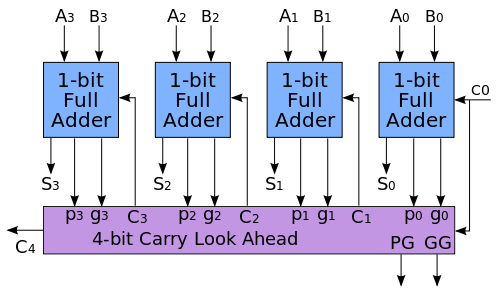
\includegraphics[width = \textwidth]{4bitcarrylookahead} $$ 

Group Propagate and Group Generate $$ \begin{aligned} 
C_4 &= G_3 + G_2 \cdot P_3 + G_1 \cdot P_2 \cdot P_3 + G_0 \cdot P_1 \cdot P_2 \cdot P_3 + C_0 \cdot P_0 \cdot P_1 \cdot P_2 \cdot P_3 \\ 
P_G  &= P_3 \cdot P_2 \cdot P_1 \cdot P_0 \\
GG &= G_3 + G_2 \cdot P_3 + G_1 \cdot P_2 \cdot P_3 + G_0 \cdot P_1 \cdot P_2 \cdot P_3
\end{aligned} $$  

Array of Logic Elements \begin{itemize} 
\item If the same combinational operations are performed on each bit of a 32 bit word(s), build an array of logic elements 
\item  32 Bit wide 2 in 1 multiplexer and compact version of 32 bit 2 in 1 multiplexer
$$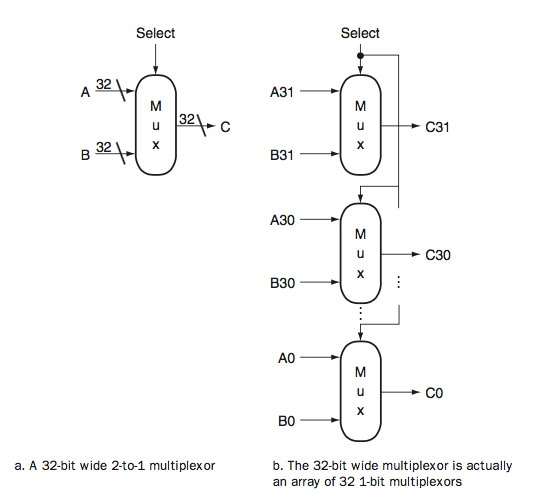
\includegraphics[width = \textwidth]{arraylogicelements}$$ 

\end{itemize} 
 
 1 Bit ALU: AND and OR Operations \begin{itemize} 
 \item Operation is 1 bit: insert ss
 \item If operation is 0, result = A AND B 
 \item If operation is 1, result = A OR B 
$$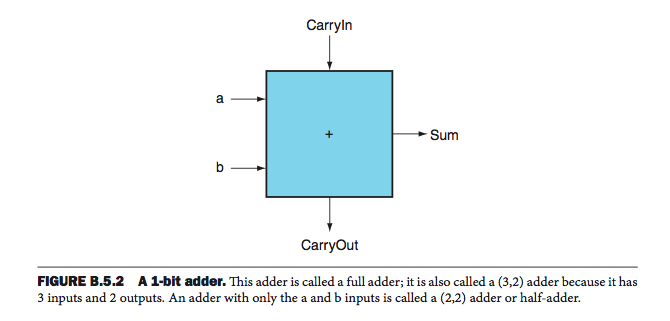
\includegraphics[width = \textwidth]{1bitadder} $$  \end{itemize} 

1 Bit ALU: AND, OR, \& Addition Operations \begin{itemize} 
\item Operation is now 2 bits 
\item If operation is 00, result = A AND B 
\item If operation is 01, result = A OR B 
\item If operation is 10, result = A + B 
$$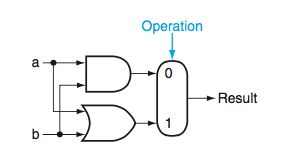
\includegraphics[width = \textwidth]{1bitlogicalunit}$$ 

\end{itemize}

1 Bit ALU: AND, OR, Addition \& Subtraction Operations \begin{itemize}
\item Operation is still 2 bits
\item If operation is 00, result = A AND B 
\item If operation is 01, result = A OR B 
\item If operation is 10, binvert is 0 and carry in (for bit 0) is 0, result = A + B 
\item If operation is 10, binvert is 1 and carry in (for bit 0) is 1, result = A  - B

\end{itemize} 

1 Bit ALU: AInvert Inclusion \begin{itemize} 
\item If operation is 00, ainvert is 1 and binvert is 1, result = A NOR B 
\item If operation is 01, ainvert is 1 and binvert is 1, result is A NAND B 
\end{itemize} 
$$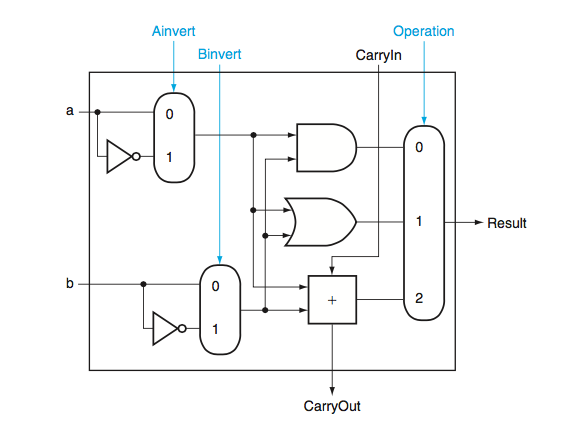
\includegraphics[width = \textwidth]{1bitALU4operationsAinvert}$$ 


Set on Less than Instruction \begin{itemize} 
\item If (A < B) then result = 1; otherwise result = 0 
\item A, B and result refer to their 32-bit wide values 
\item Computing the value of result, the ALU's full adder has to compute A - B
\item Hence, set ainvert to 0, binvert to 1 and carry in (for bit 0) to 1
\item The answer to (A - B) will be negative if (A < B) andopositive if (A $\geq$ B)
\item The 5 output of the full adder of the most significant bit (bit 31) is 1 if (A - B) is negative and 0 if (A - B) is positive 
\end{itemize} 

1 Bit ALU: Set on Less Than \begin{itemize} 
\item Used for bits 0-30 
\item The Less input is the bit's value for the SLT instruction 
$$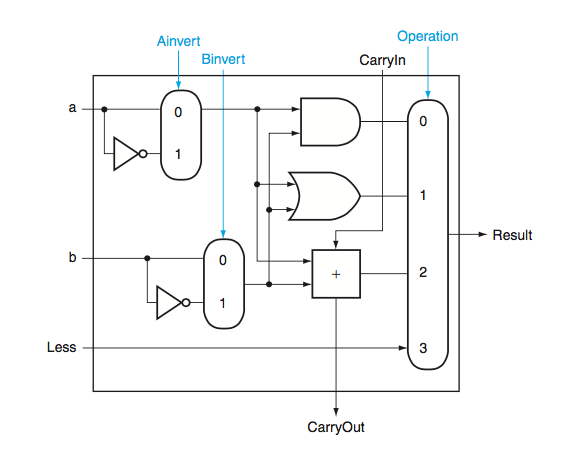
\includegraphics[width = \textwidth]{1bitALUlessthan}$$ 
$$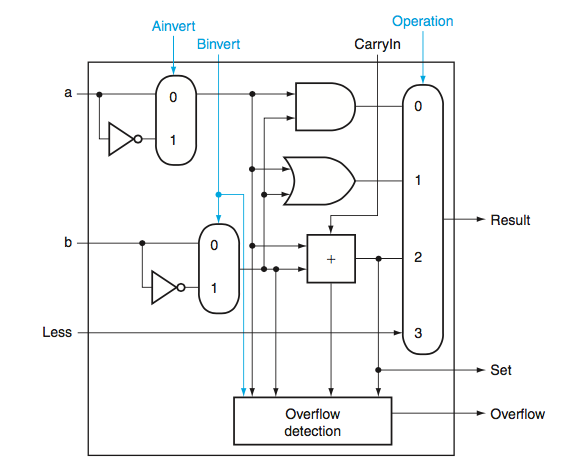
\includegraphics[width = \textwidth]{1bitALUlessthanoverflow}$$ 


\end{itemize} 

1 Bit ALU for bit-31 (insert pic) \begin{itemize} 
\item Includes circuitry for overflow detection (overflow) and a value (set) for SLT
\item The Less input is is this bit's value for the SLT instruction 
 \end{itemize} 
 
 32 Bit ALU \begin{itemize} 
 \item If operation is 11, ainvert is 0, binvert is 1, and carry in (for bit 0) is 1, then
 \item If A < B. then result is 1; otherwise result = 0
 \item The Zero output of the ALU is 1 if all 32 bits of the result are 0; otherwise Zero is 0
 \end{itemize} 
 
 32 Bit ALU Black Box \begin{itemize} 
 \item A, B and result are 32 bit wide 
 \item Zero, Overflow and carry out are 1 bit 
 \item ALU operations is 4 bit wide 
 \item The 4 bits of ALU operations are ainvert, binvert, and the 2 operation bits of the ALU design 
 $$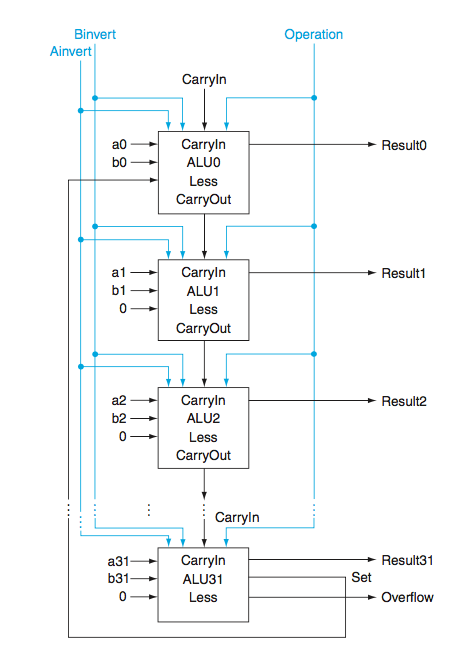
\includegraphics[scale = 0.8]{32bitALU}$$ 

 \end{itemize} 
 
 ALU Operations $$\begin{tabular}{|c|c|} \hline
 ALU Operations & Functions \\ \hline 
 0000 & AND \\ \hline 
 0001 & OR \\ \hline 
 0010 & add \\ \hline 
 0110 & subtract \\ \hline
 0111 & set on less than \\ \hline 
 1100 & NOR \\ \hline \end{tabular} $$ 
$$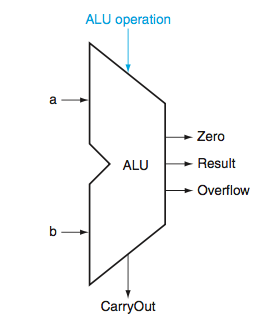
\includegraphics[scale = 0.5]{ALU}$$ 



\end{document}